\chapter{Hipoteza}

Statistička je hipoteza tvrdnja o parametru jedne ili vise populacija.\cite{matstat} Npr. tvrdnja da prosjecan broj jabuka pojedenih na dan iznosi 2 je validna hipoteza.

\begin{itemize}
\item Nul hipoteza \textit{(eng. null hypothesis)} $H_0$
\item Alternativna hipoteza \textit{(eng. alternative hypothesis)} $H_a$
\end{itemize}

\section{Nul hipoteza}

Nul je hipoteza \textit{(eng. null hypothesis)} teza o populaciji.

Ona može biti donesena na temelju modela tog sustava (npr. kroz biološke, fizikalne, matematičke ili druge zakonitosti), empirijska mjerenja sustava te na mnoge druge načina. 

U većini literature \cite{matstat}\cite{vis3} se označava s $H_0$. Primjeri nul hipoteza mogu biti razne, od hipoteza očekivanja populacije, hipoteza udjela subpopulaciju u populaciji, i mnoge druge primjene.

\section{Alternativna hipoteza}
%Testiranje ne radi je li nešto točno ili nije. Ja vidim samo crno bijelo kroz naočale dok ono u stvarnosti može biti i rozo. U postupku nessto prihvaćamo ili odbacujemo s nekim određenim rizicima. Bez obzira na ishod testa.

No sto ako postupkom testiranja odbacujemo nul hipotezu? Onda prihvaćamo alternativnu hipotezu. To naravno ne implicira u apsolutnu točnost jer na temelju rezultata dobivenih u uzorku ne možemo nikad biti sasvim sigurni je li odabrana
hipoteza ispravna ili ne. \cite{vis3}

Neka je $H_0:$ \emph{Varijanca bodova na SISu je 15}. tj. $H_0:\; \sigma^2 = 15$. Sto bi bila alternativna hipoteza? 

Logično negacija $H_0$ te je time $H_a:\; \sigma^2 \ne 15$. Ovo je dvostrana alternativna hipoteza jer parametar $\sigma^2$ u alternative može biti i veći i manji od nul hipoteze. 

Postoji još jedna mogućnost alternativne hipoteze, a to je jednostrana. Glasi ovako: $H_a:\; \sigma^2 > 15$ ili $H_a:\; \sigma^2 < 15$. Kao sto vidimo ova alternativna hipoteza gleda samo jednu stranu toga parametra te se zato zove jednostavna. \cite{engstat}

Kada rabimo koju? Jednostranu rabimo samo ako smo iznimno uvjereni da je suprotan slučaj nemoguć, zbog fizikalnih, matematičkih ili ostalih zakona. Stoga najčešće uzimamo dvostranu alternativnu hipotezu.

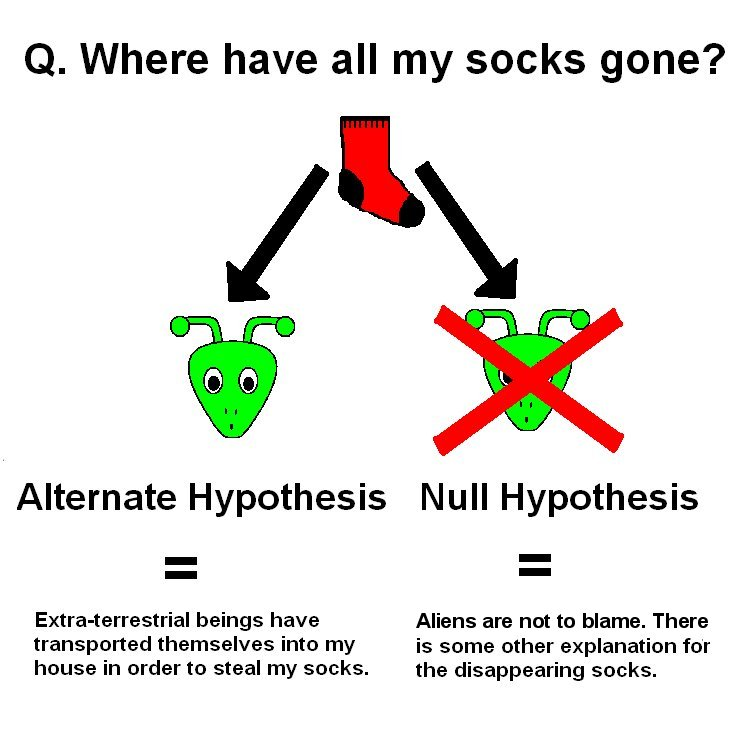
\includegraphics[width=8.2cm]{aliens.jpg}